\section*{Evaluation}
Evaluation of segmentation algortihm,s has long been done by comparing the rpedictions to a ground thruth, masks of cells drawn by humans, usually professionals in that area, as seen in Mesmer the TissueNet was done by crowd-sourcing the workload. This aproach has many short comings, the most obvious one that we have to trust the decisions made by the professional, and verifiyng independently requires euqally uncertain work. distinguishing between cell, nucleus, ecm, and ohter structures is often a heuristic task. nonetheless the quality of human segmentation exceeded CV, in in many cases continues to, but we arrive at limitations quit quickly especially in  dense tissue like the spleen. such compact organs complicate basic staining techniques, resulting in sub-par membrane and ribosome stains required for unubiquitous segmentation \ref{fig:focusBCMY}. to not rely on a difficult to verify groundtruth [I] included two additional methods of evaluation. on is based on principal component analyssis (PCA), using the input-image, on which the segmentation was performed, to calculate metric that indicate a 'good' segmentation. the other simply compares the predictions among each other | this of course does not tell which is the colsest to a human-identifiable truth, but which algorithm provides a stable predictip of the cells. this difficulty of segmentation is extended when discussing 3d segmentation. 
\begin{figure}
    \centering
    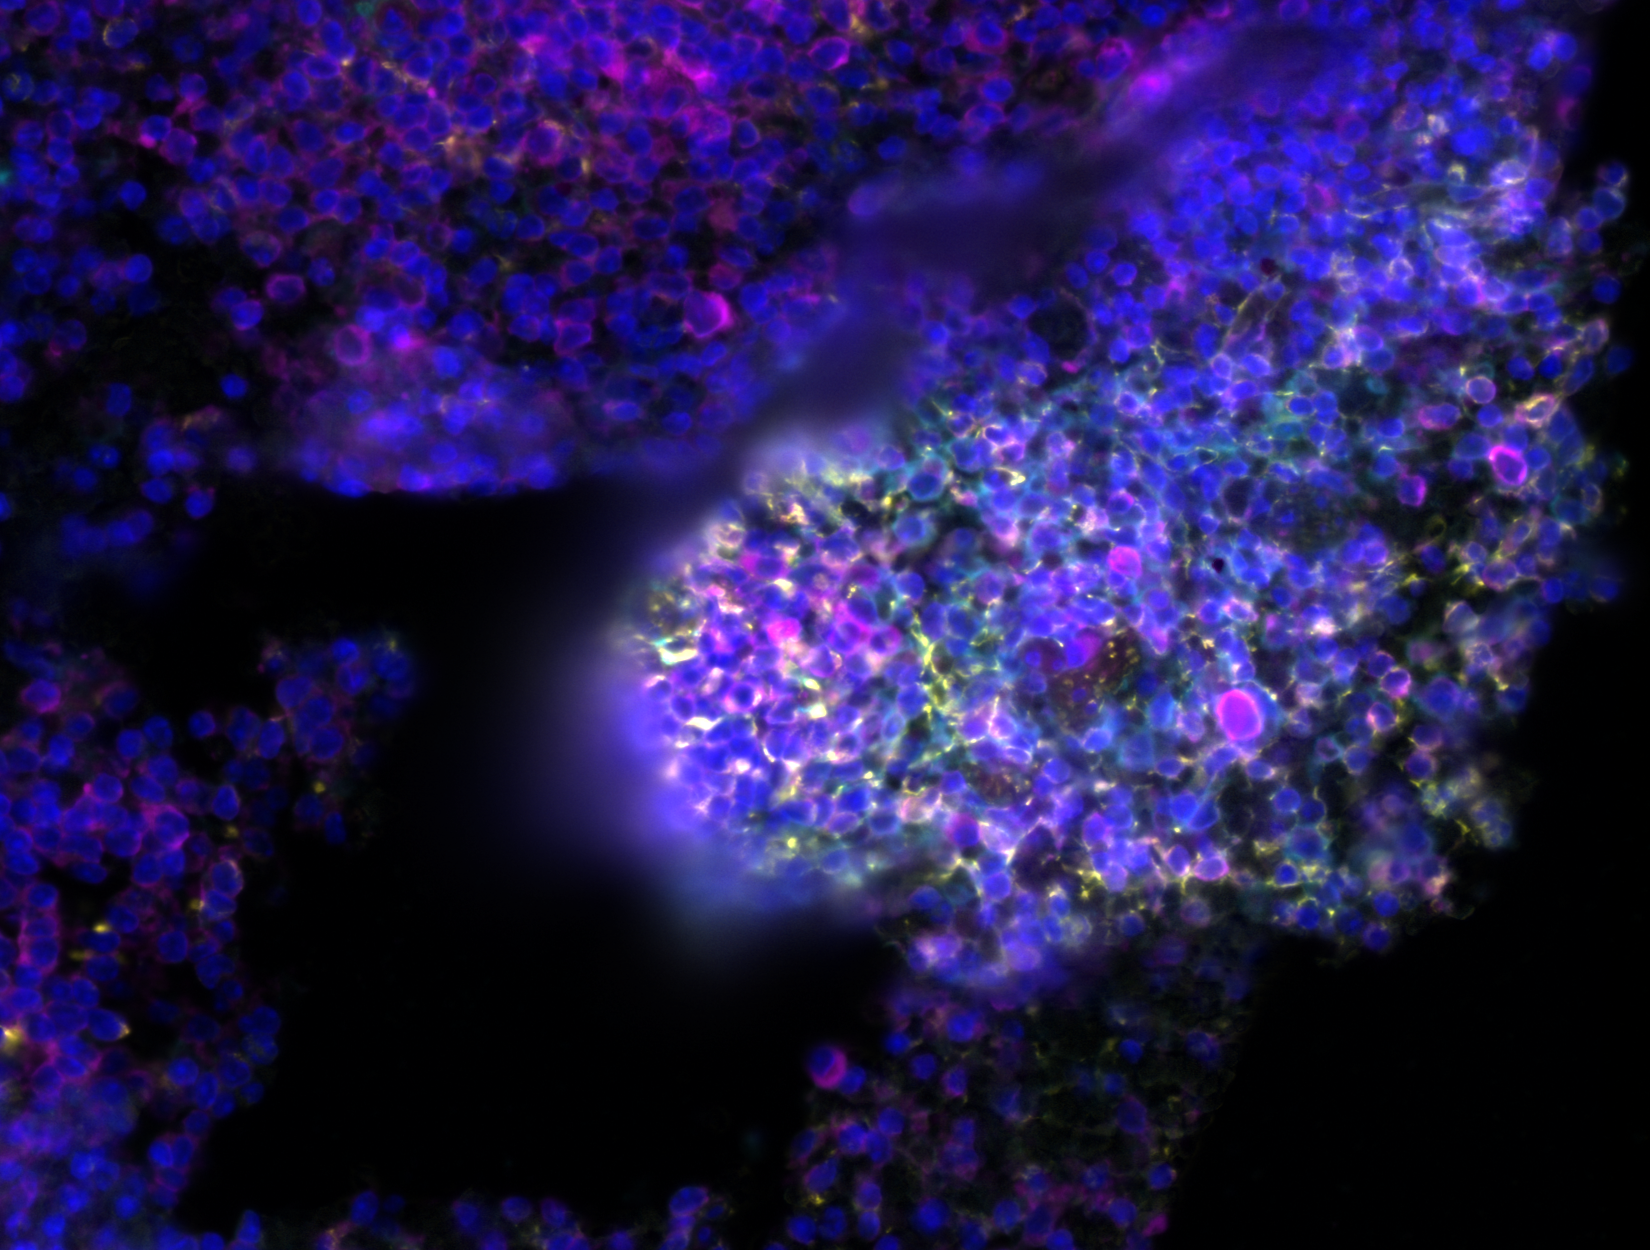
\includegraphics[width=0.5\linewidth]{Images/focus_BCMY.png}
    \caption{The region with the best/usable membrane-stain. red: dapi, green:atp/adhesin, blue: ribo}
    \label{fig:focusBCMY}
\end{figure}
% 
\subsection*{Reference Based}
we make mask. mask bad. but o well.
\begin{figure}
    \centering
    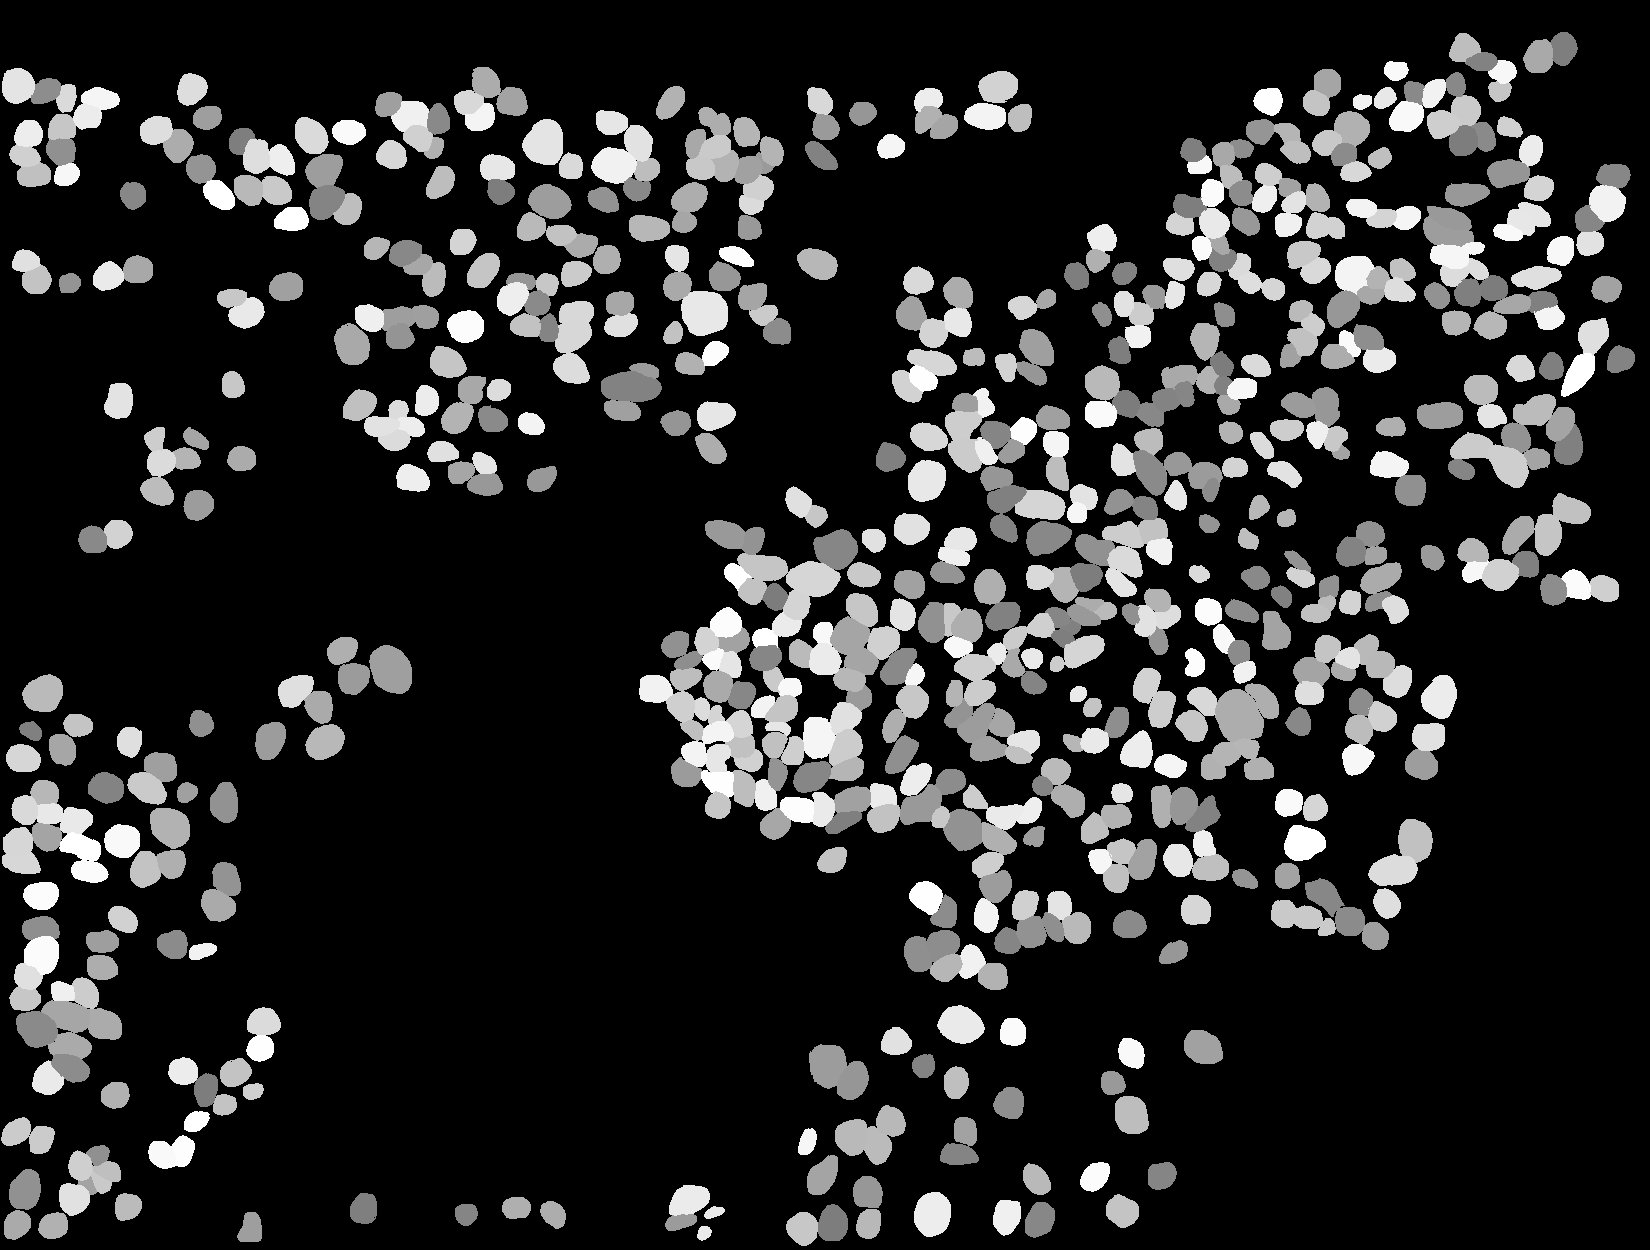
\includegraphics[width=0.5\linewidth]{Images/eval/TMA2_13-3_whole-cell_labels.jpg}
    \caption{Segmentation mask used for eval. Cell masks drawn by hand in FIJI/Labkit}
    \label{fig:CellMask}
\end{figure}
% 
% 
\begin{figure}
    \centering
    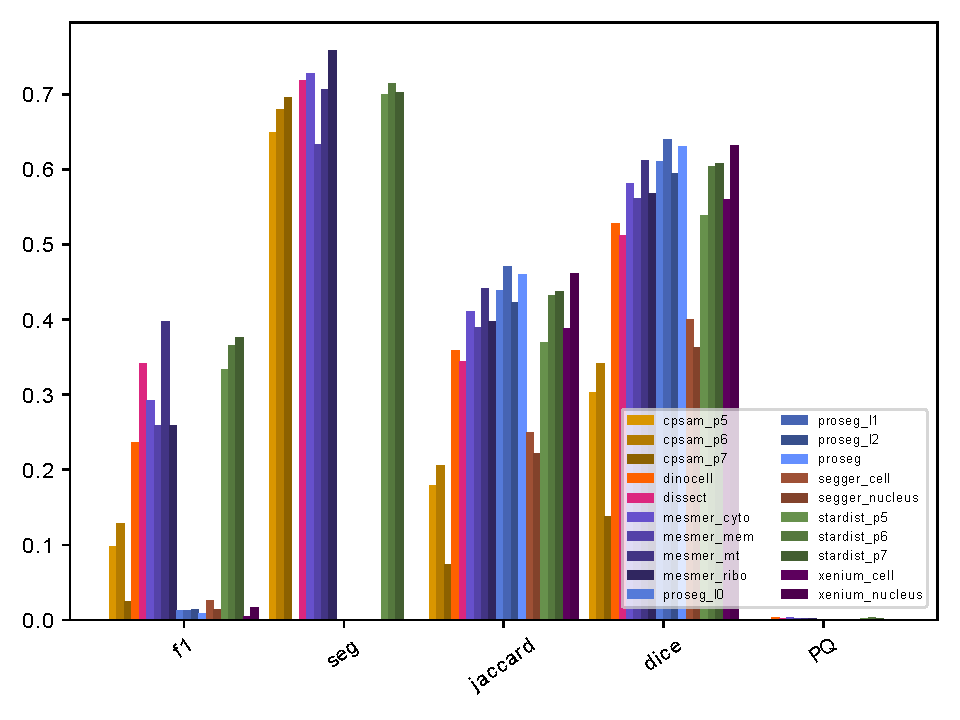
\includegraphics[width=0.5\linewidth]{Images/eval/cs_bars_legend.pdf}
    \caption{Bar plot of the different metrics offered by the CS-Benchmark package.}
    \label{fig:cs-bars}
\end{figure}
\begin{figure}
    \centering
    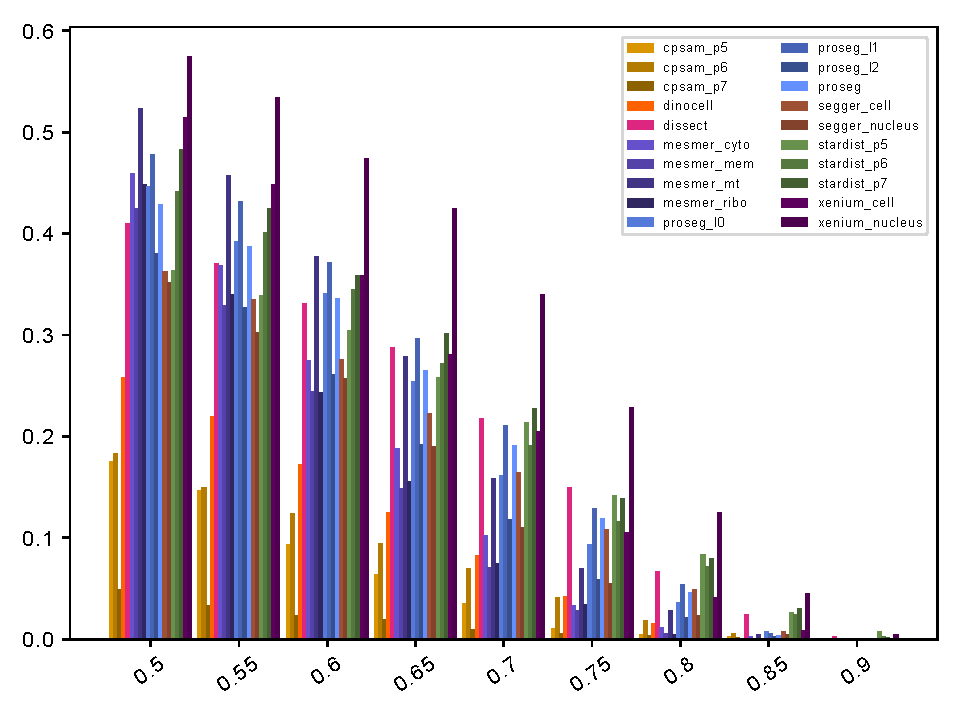
\includegraphics[width=0.5\linewidth]{Images/eval/u4n_bars_legend.pdf}
    \caption{Bar plot of the F1 value at increasing thresholds. Calculated using unet4nuclei's evaluation methods.}
    \label{fig:u4n-bars}
\end{figure}

\subsection*{Reference Free}
Since computer vision can theoretically and practically often does outperform human-con--- human segmentation and in somecases human-consensus (cellpose) - meaning using references is bound to stop working soon.. methods evaluationg based on statistics extracted form the image to segment on or by finding a groundtruth determined by the highest probability of a mix of segmentation results. see overnext section.
\subsubsection*{CellSegmentationEvaluator}
On homogeneity of cell types (KMeans):
cell types should be roughly similar in composition across all channels
cell types can be approximated by cell clusters
the average CV across all clusters for a given number of clusters is a proxy for similarity in composition within cell types
averaging the average CV across all clusters across different numbers of the cluster is also a proxy for similarity in composition within cell types
% 
s. Cell types were defined using KMeans clustering performed on the mean cell intensities across all channels after applying z-score standardization for each channel
K, number of cell types, varied from 1 to 10
% 
On homogeneity of cell types (PCA):
and (b) as before
(c)  the fraction of variance accounted for by the first principal component 
of the cells in each cluster is a proxy for similarity in composition of each cell type
(d)  averaging this fraction over different numbers of clusters is also a proxy for similarity of each cell type
% 
An important consideration to note is that our metrics are based in large part on the assumption that tissue images used for evaluation contain different cell types that vary in their expression of different markers. If a tissue image is largely uniform, then our measures of segmented cell homogeneity will yield similar results regardless of the accuracy of cell segmentation masks. The greater the number of channels measured and the larger the differences between cell types, the more discriminating our metrics will be.
% 
The metrics also do not make any assumptions about allowable cell shapes. Measuring cell shape is an inherent problem for 2D tissue images where 3D cells are only seen in a thin layer in the z-axis. Cells belonging to the same cell type might be captured at different angles or heights and therefore display different shapes. Although our metrics of homogeneity at the cell level solve this issue indirectly (since cells from the same cell type but at different views should have similar channel compositions), segmentation methods that produce cells and nuclei with unexpected shapes are not directly penalized.
% 
\begin{table}[H]
    \centering
    \caption{CellSegmentationEvaluation. Results for Mesmer, Segger, Xenium.}
    \begin{tabular}{l|c|c|c|c|c}
         Metrics & mt & mem & ribo & Segger & Xenium \\
         \hline
         Quality Score & \textbf{2.707} & \textbf{2.941} & \textbf{2.976} & \textbf{1.603} & \textbf{2.251} \\
         \hline
         NC & 1.104 & 1.113 & 1.135 & 0.236 & 0.264 \\
         \hline
         FFC & 0.659 & 0.772 & 0.760 & 0.259 & 0.746 \\
         1-FBC & 0.935 & 0.930 & 0.933 & 0.993 & 0.920 \\
         FCF & 0.956 &  0.960 & 0.961 & 0.987 & 0.953\\
         \hline 
         FMCN & 0.948 & 0.955 & 0.963 & 0.759 & 0.932 \\
         \hline
         1/(ACVF+1) & 0.542 & 0.528 & 0.479 & 0.441 & 0.493\\
         FPCF & 0.616 & 0.650 & 0.624 & 0.533 & 0.648\\
         \hline
         1/(ACVC+1)& 0.626 & 0.629 & 0.620 & 0.702 & 0.774 \\
         FPCC & 0.453 & 0.457 & 0.447 & 0.450 & 0.425\\
         AS & 0.263 & 0.258 & 0.258 & 0.244 & 0.255\\
         \hline
         1/(ln(CSSD)+1) & 0.142 & 0.139 & 0.141 & 0.134 & 0.127\\
    \end{tabular}
    \label{tab:PCA}
\end{table}
% \subsubsection*{PB}
% big MAYBE
\subsubsection*{Cross-Evaluation}
To see which algorithm compares well, while the others are less consistent.
% \begin{figure}
%     \centering
%     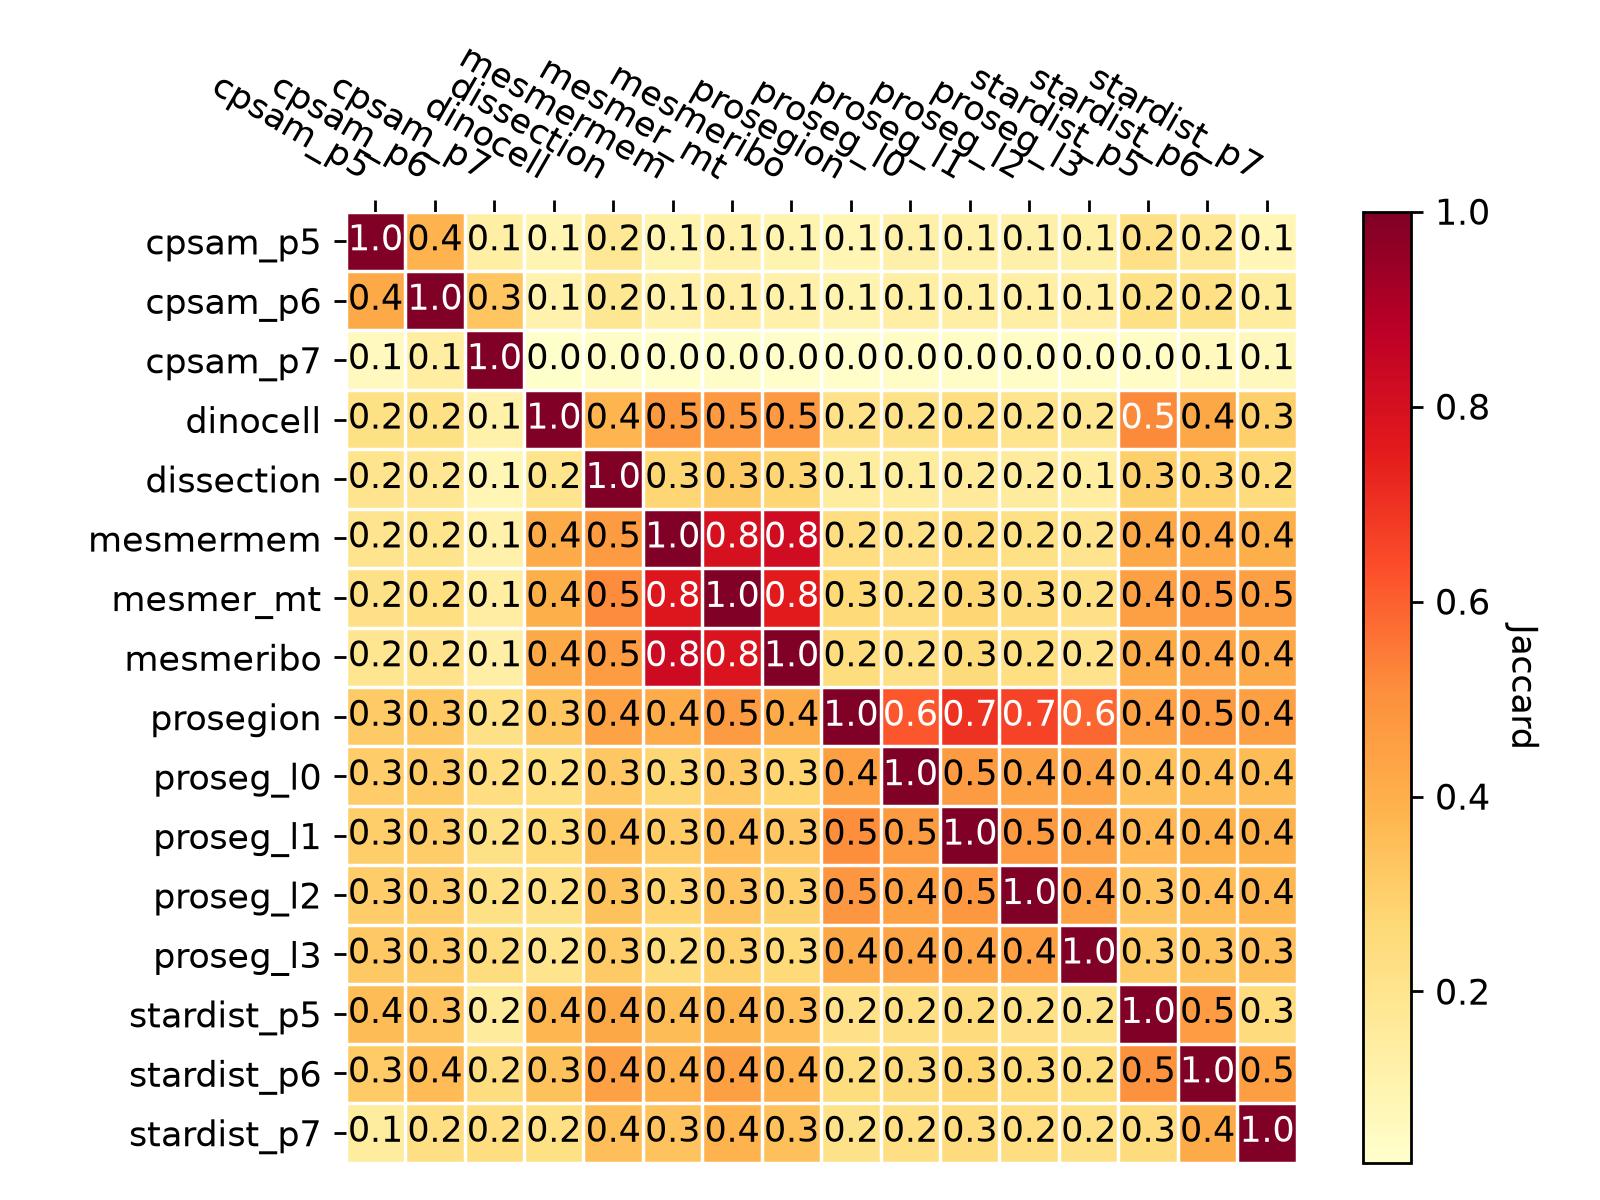
\includegraphics[width=0.5\linewidth]{Images/eval/cross_af1_Jaccard_newmem.png}
%     \caption{Cross Evaluation using unet4nuclei's Jaccard method.}
%     \label{fig:af1_IoU}
% \end{figure}
% \begin{figure}
%     \centering
%     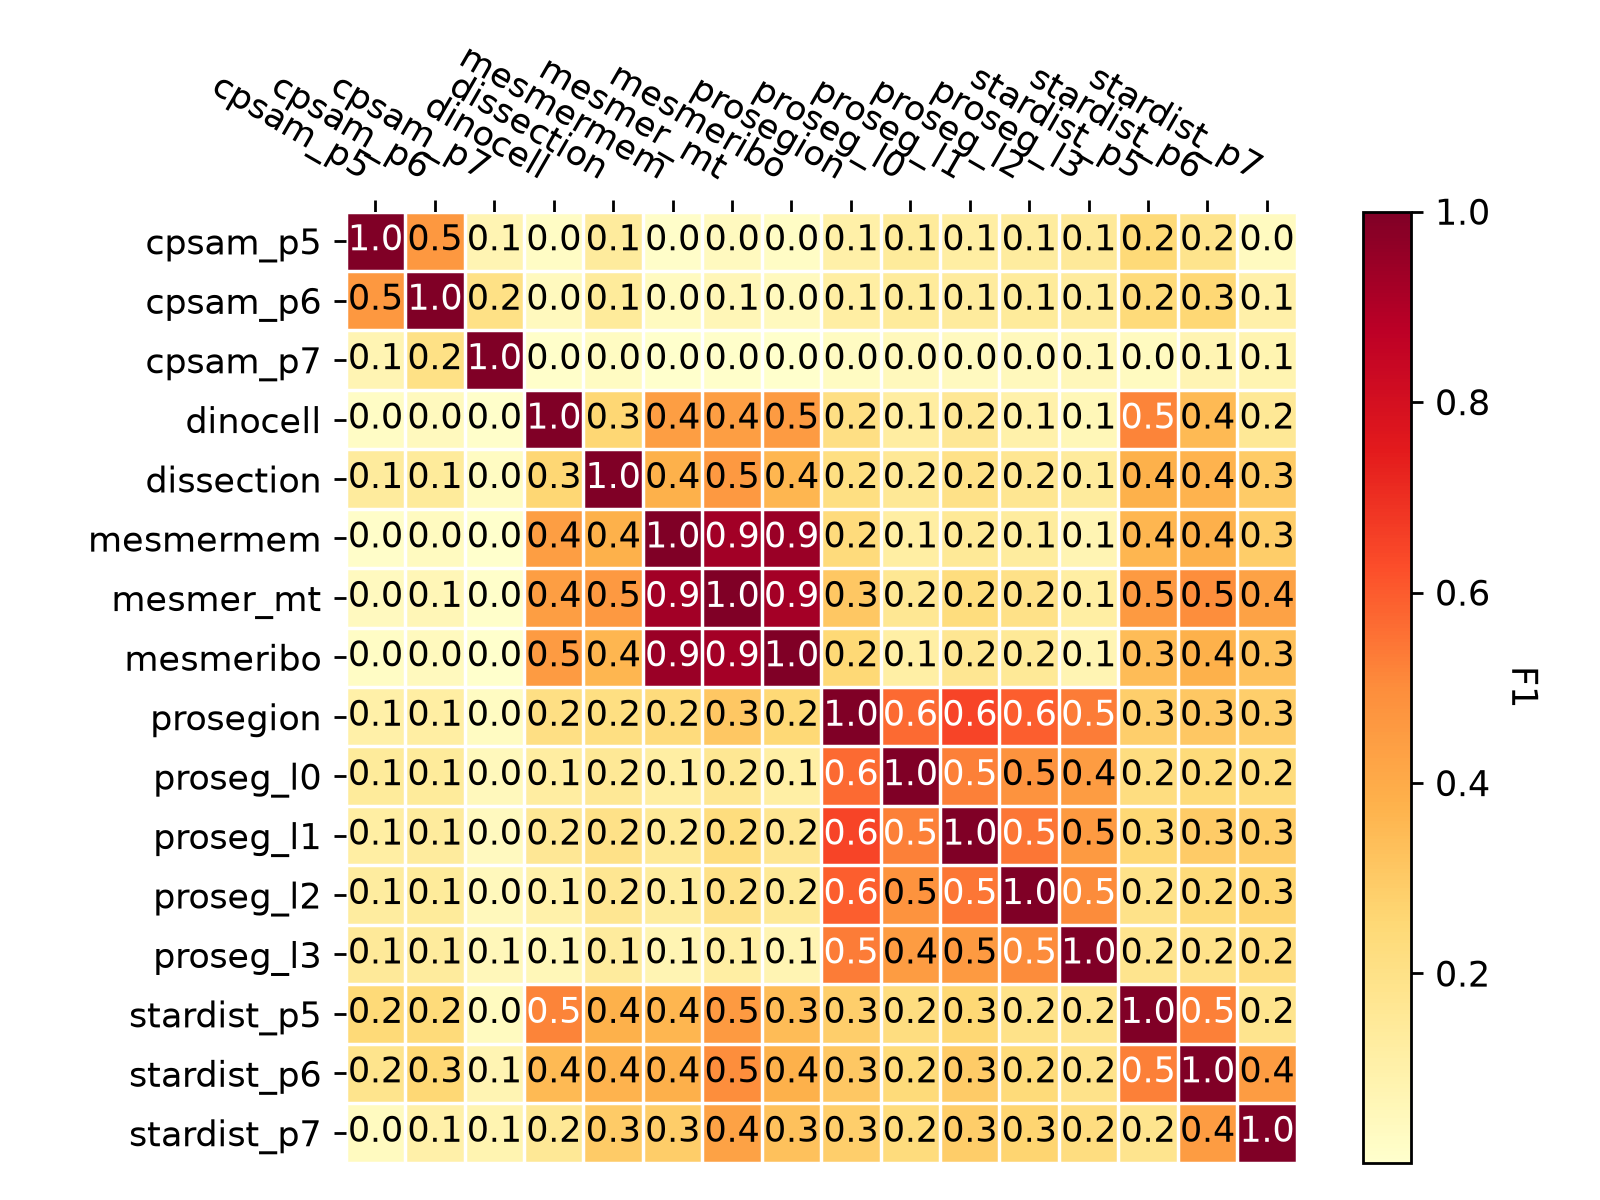
\includegraphics[width=0.5\linewidth]{Images/eval/cross_af1_F1_newmem.png}
%     \caption{Cross Evaluation using unet4nuclei's F1 method.}
%     \label{fig:af1_F1}
% \end{figure}
% \begin{figure}
%     \centering
%     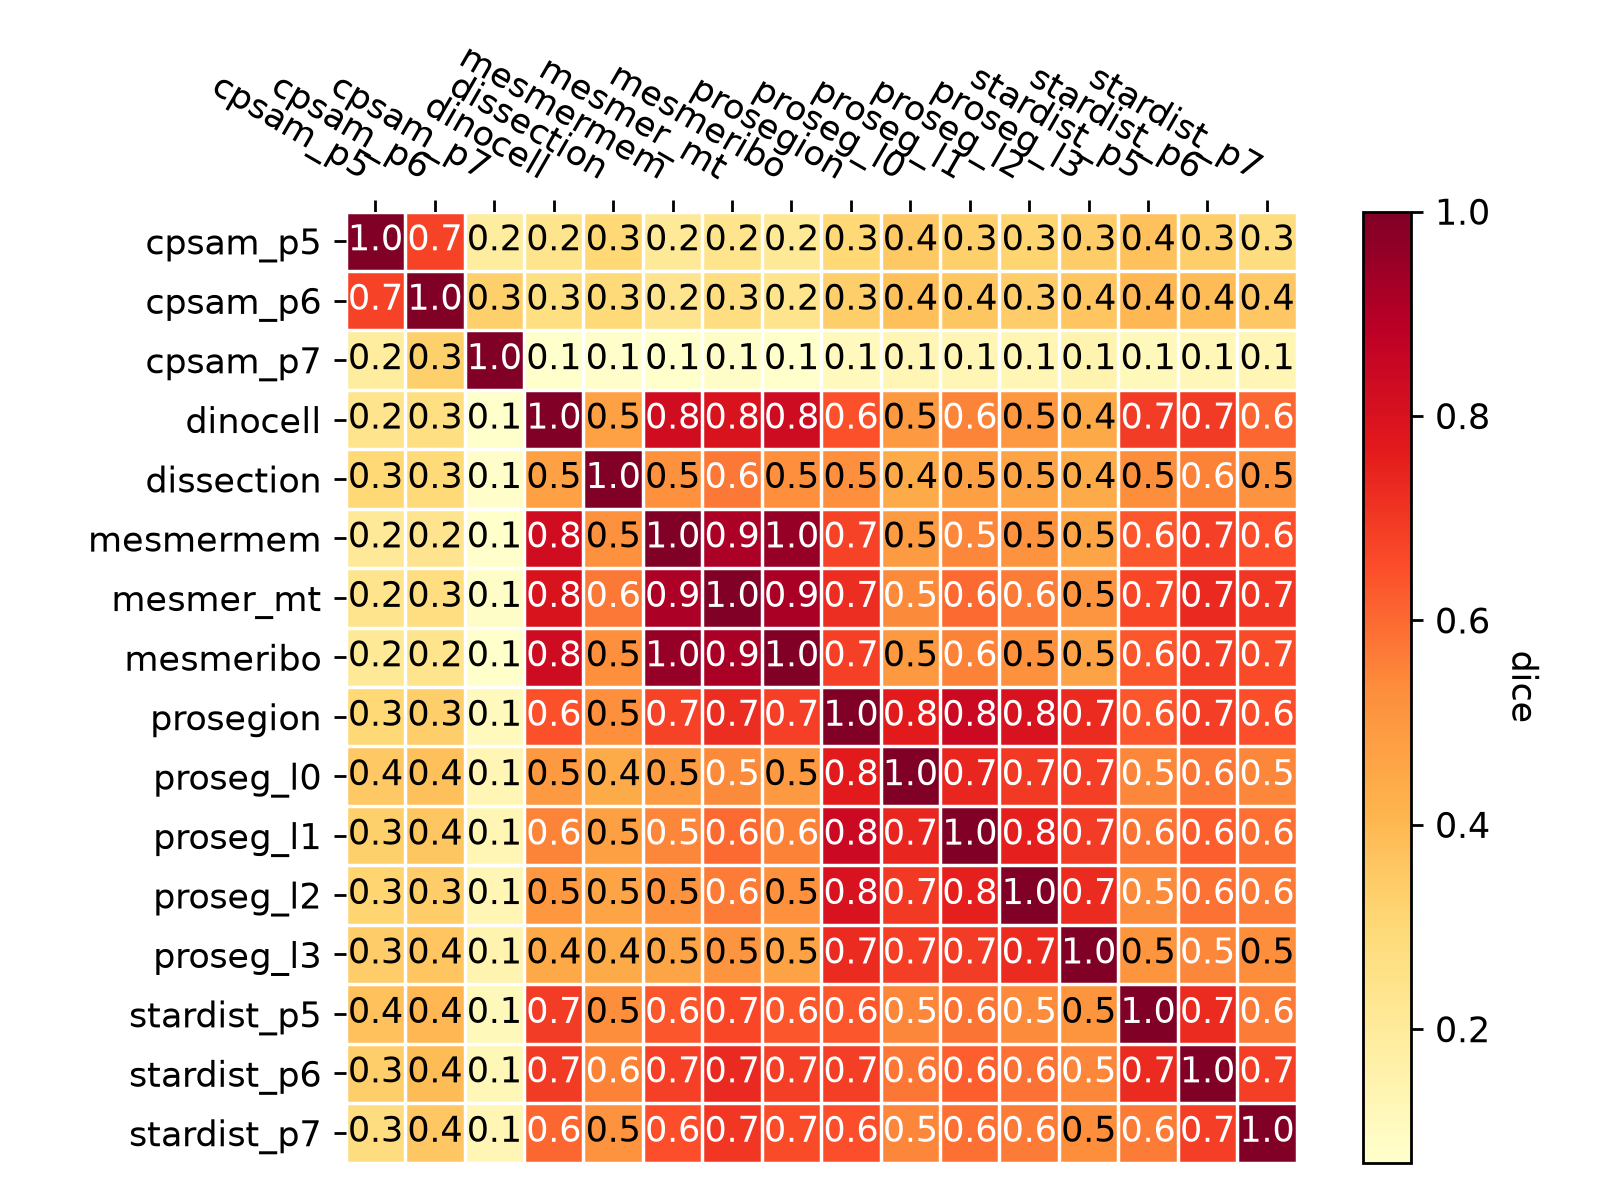
\includegraphics[width=0.5\linewidth]{Images/eval/cross_cs_dice_all.png}
%     \caption{CS-Benchmark's Dice method.}
%     \label{fig:cs_dice}
% \end{figure}
\begin{figure}
    \centering
    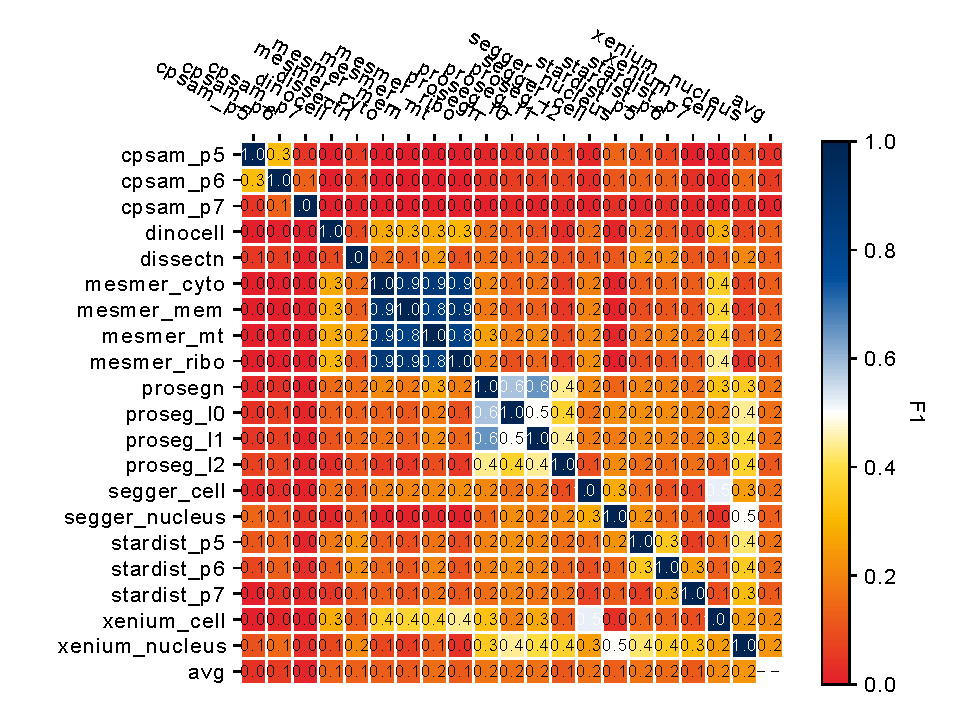
\includegraphics[width=0.5\linewidth]{Images/eval/F1_u4n_cross_evaluation_newmem_font.pdf}
    \caption{Cross Evaluation using unet4nuclei's F1 method.}
    \label{fig:u4n_jac}
\end{figure}
\begin{figure}
    \centering
    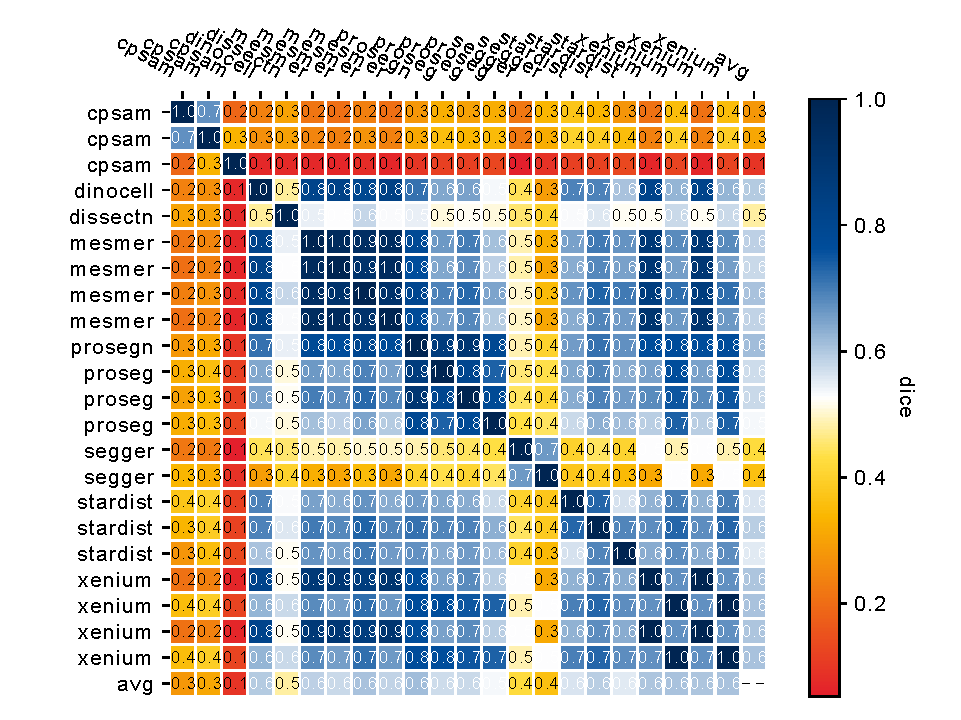
\includegraphics[width=0.5\linewidth]{Images/eval/dice_cs_cross_evaluation_newmem_font.pdf}
    \caption{Cross Evaluation using CS-Benchmark's DCE value.}
    \label{fig:placeholder}
\end{figure}